\vspace{-10pt}
\section{Experimental Results}
\vspace{-5pt}
\subsection{Experimental Settings}
\vspace{-5pt}
In order to evaluate \textsf{\small PCStream}, we have implemented it in the
Linux kernel (version 4.5) on a PC host with Intel Core i7-2600 8-core
processor and 16~GB DRAM.  As a multi-streamed SSD, we used Samsung's PM963
480~GB SSDs.  The PM963 SSD supports up to 9 streams; 8 user-configurable
streams and 1 default stream.  When no stream is specified with a write
request, the default stream is used.  To support internal streams, we have
modified the existing PM963 FTL firmware.  For a detailed performance analysis,
we built a modified {\tt nvme-cli}~\cite{nvmecli} tool that can retrieve the internal
profiling data from \textsf{\small PCStream}-enabled SSDs.  
Using the modified {\tt nvme-cli} tool, we can monitor 
WAF values and per-block data lifetimes from the extended PM963 SSD during run time.

We compared \textsf{\small PCStream} with three existing schemes:
\textsf{\small Baseline}, \textsf{\small ManualStream}~\cite{MultiStream}, and
\textsf{\small AutoStream}~\cite{AutoStream}.  \textsf{\small Baseline}
indicates a legacy SSD that does not support multiple streams. \textsf{\small
ManualStream} represents a multi-streamed SSD with manual stream allocation.
\textsf{\small AutoStream} represents the LBA-baed stream management technique
proposed in ~\cite{AutoStream}. 


We have carried out experiments with various benchmark programs
which represent distinct write characteristics.
RocksDB~\cite{RocksDB} and Cassandra~\cite{Cassandra} have
append-only write patterns. SQLite~\cite{SQLite} has in-place update write patterns
and GCC~\cite{GCC} has write-once patterns.  
For more realistic evaluations, we also used mixed workloads running two 
different benchmark programs simultaneously.

In both RocksDB and Cassandra experiments, Yahoo! Cloud Serving Benchmark
(YCSB)~\cite{YCSB} with 12-million keys was used to generate update-heavy
workloads (workload type A) which consists of 50/50 reads and writes.  Since
both RocksDB and Cassandra are based on the append-only LSM-tree
algorithm~\cite{LSM}, they have three dominant I/O activities (such as logging,
flushing, and compaction).  Cassandra is written in Java, so its PC is
extracted by the modified procedure described in Section 5.4.  In SQLite evaluations,
TPC-C~\cite{TPCC} was used with 20 warehouses.  SQLite has two dominant I/O
activities such as logging and updating tables.  In GCC experiments, a Linux
kernel was built 30 times.  For each build, 1/3 of source files, which were
selected randomly, were modified and recompiled.  Since GCC creates many
temporary files ({\it e.g.}, \texttt{.s}, \texttt{.d}, and \texttt{.rc}) as
well as long-lived files ({\it e.g.}, \texttt{.o}) from different compiler
tools, there are more than 20 dominant PCs.  To generate mixed workloads, we run
RocksDB and GCC scenarios together (denoted by Mixed 1), and run SQLite and GCC
scenarios at the same time (denoted by Mixed 2).  In order to emulate an aged
SSD in our experiments, 90\% of the total SSD capacity was initially filled up
with user files before benchmarks run.

\vspace{-10pt}
\subsection{Performance Evaluation}
\vspace{-5pt}

\begin{figure}[t]
	\centering
	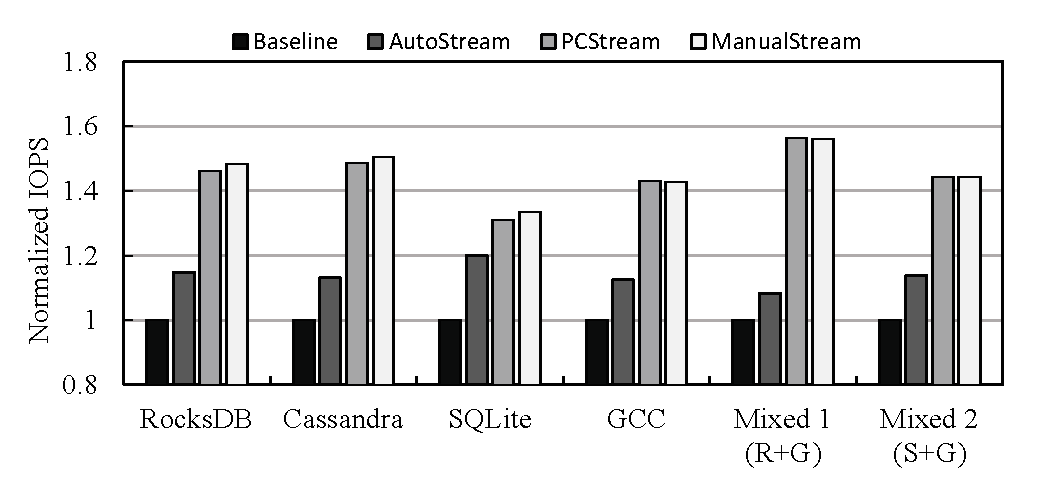
\includegraphics[width=0.95\linewidth]{figure/iops}
	\caption{A comparison of normalized IOPS.}
	\vspace{-5pt}
	\label{fig:iops}
	\vspace{-10pt}
\end{figure}

We compared IOPS values of three existing techniques with \textsf{\small
PCStream}.  Fig.~\ref{fig:iops} shows normalized IOPS for six benchmarks with
four different techniques. For all the measured IOPS values\endnote{ For
RocksDB, Cassandra, and SQLite, the YCSB benchmark and TPC-C benchmark compute
IOPS values as a part of the benchmark report.  For GCC,
where an IOPS value is not measured during run time, 
we computed the IOPS value as a ratio between the total number of write requests
(measured at the block device layer) and the total elapsed time of running GCC.},
\textsf{\small PCStream} improved the average IOPS by 45\% and 28\% over 
\textsf{\small Baseline} and \textsf{\small AutoStream}, respectively.
\textsf{\small PCStream} outperformed \textsf{\small AutoStream}
by up to 56\% for complex workloads ({\it i.e.}, GCC, Mixed1 and Mixed 2) where
the number of extracted PCs far exceeds the number of supported streams
in PM963. The high efficiency of \textsf{\small PCStream} under complex
workloads comes from two novel features of \textsf{\small PCStream}: (1) LBA-oblivious 
PC-centric data separation and (2) a large number of streams supported 
using internal streams. \textsf{\small AutoStream}, on the other hands,
works poorly except for SQLite where the LBA-based separation
can be effective.
Even in SQLite, \textsf{\small PCStream} outperformed \textsf{\small AutoStream}
by 10\%.

\vspace{-10pt}
\subsection{WAF Comparison}
\vspace{-5pt}

Fig.~\ref{fig:waf} shows WAF values of four techniques for six benchmarks.
Overall, \textsf{\small PCStream} was as efficient as \textsf{\small
ManualStream}; Across all the benchmarks, \textsf{\small PCStream} showed 
similar WAF values as \textsf{\small ManualStream}. \textsf{\small PCStream}
reduced the average WAF by 63\% and 49\% over \textsf{\small Baseline} and
\textsf{\small AutoStream}, respectively.  

As expected, \textsf{\small Baseline} showed the worst performance among all
the techniques. Owing to the intrinsic limitation of LBA-based data
separation, \textsf{\small AutoStream} performs poorly except for
SQLite.  Since \textsf{\small PCStream} (and \textsf{\small ManualStream}) did
not depend upon LBAs for stream separations, they performed well consistently,
regardless of write access patterns. As a result, \textsf{\small PCStream}
reduced WAF by up to 69\% over \textsf{\small AutoStream}.

%Only SQLite had in-place update patterns for log files, 
%but the larger amount of data were written to database files 
%whose lifetimes are determined by the client
%which makes hard to predict their lifetime by the address.  In PCStream,
%however, long-lived data in database files are moved to internal streams during
%GC so that we can further reduce WAF.

One interesting observations in Fig.~\ref{fig:waf} is that \textsf{\small
PCStream} achieved a lower WAF value than even \textsf{\small ManualStream} for
GCC, Mixed 1, and Mixed 2 where more than the maximum number of streams in
PM963 are needed.  In \textsf{ManualStream}, DB applications and GCC were
manually annotated at offline, so that write system calls were statically bound
to specific streams during compile time.  When multiple programs run together
as in three complex workloads ({\it i.e.}, GCC, Mixed 1 and Mixed 2), static stream
allocations are difficult to work efficiently because they cannot adjust to
dynamically changing execution environments.  However, unlike \textsf{\small
ManualStream}, \textsf{\small PCStream} continuously adapts its stream
allocations during run time, thus quickly responding to varying execution
environments.

\begin{figure}[t]
	\centering
	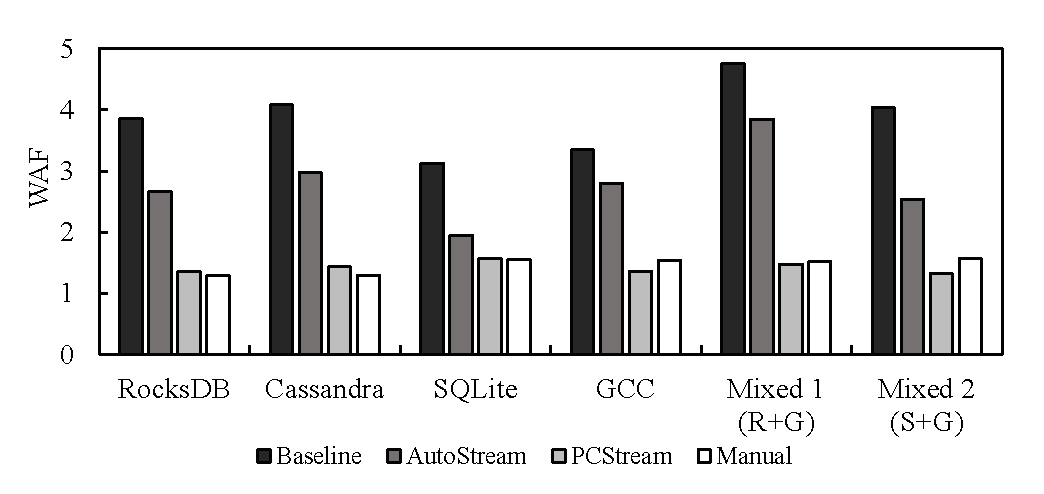
\includegraphics[width=1.\linewidth]{figure/waf}
	\caption{A comparison of WAF under different schemes.}
	\vspace{-5pt}
	\label{fig:waf}
	\vspace{-10pt}
\end{figure}


%since the Manual scheme has static stream allocation.
%In Manual, once data types is mapped to the stream, the mapping is not changed 
%during runtime.
%For complex workloads which have large number of PCs such as mixed cases,
%it is difficult to expect data lifetimes in detail based on the data types.
%If the lifetime pattern is changed during runtime or the programmer choose
%second best stream mapping,
%Manual scheme lose the potential benefit in reducing WAf.
%However, the reclustering enables PCStream to adapt changing workload or find
%better stream mapping.
%The detailed analysis will be shown in the following subsections.
\vspace{-10pt}
\subsection{Per-stream Lifetime Distribution Analysis}

To better understand the benefit of \textsf{\small PCStream} on the WAF
reduction, we measured per-stream lifetime distributions for the Mixed 1
scenario.  Fig.~\ref{fig:distribution} shows a box plot of data lifetimes from
the 25th to the 75th percentile.  As shown in Fig.~\ref{fig:distribution},
streams in both \textsf{\small PCStream} and \textsf{\small ManualStream} are
roughly categorized as two groups, $G1$ = $\{S_1$, $S_2$, $S_3$, $S_4$, $S_5\}$
and $G2$ = $\{S_6$, $S_7$, $S_8\}$, where $G1$ includes streams with short
lifetimes and small variances ({\it i.e.}, $S_1$, $S_2$, $S_3$, $S_4$, and $S_5$) and
$G2$ includes streams with large lifetimes and large variances ({\it i.e.}, $S_6$,
$S_7$, and $S_8$). The $S_0$ does not belong to any groups as it is assigned to
requests whose lifetimes are unknown.  Even though the variance in the $S_0$ is
wider than that in \textsf{\small ManualStream}, \textsf{\small PCStream}
showed similar per-stream distributions as \textsf{\small ManualStream}.  In
particular, for the streams in $G2$, \textsf{\small PCStream} exhibited smaller
variance than \textsf{\small ManualStream}, which means that \textsf{\small
PCStream} separates cold data from hot data more efficiently.  Since
\textsf{\small PCStream} moves long-lived data of a stream to its internal
stream, the variance of streams with large lifetimes tend to be smaller over
\textsf{\small ManualStream}.

\begin{figure}[t]
	\centering
	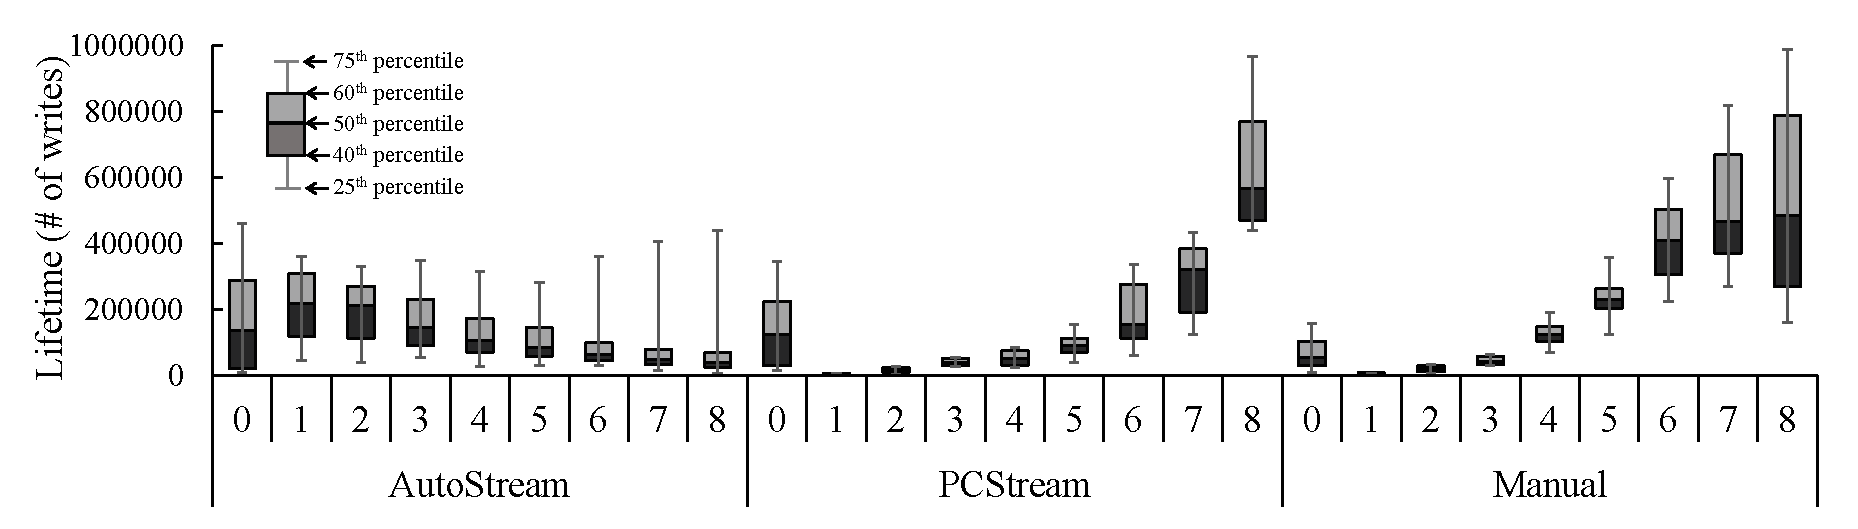
\includegraphics[width=1\linewidth]{figure/distribution}
	\caption{A Comparison of per-stream lifetime distributions.}
	\label{fig:distribution}
	\vspace{-15pt}
\end{figure}


\textsf{\small AutoStream} was not able to achieve small per-stream variances
as shown in Fig.~\ref{fig:distribution} over \textsf{\small PCStream} and
\textsf{\small ManualStream}.  As shown in Fig.~\ref{fig:distribution}, all the
streams have large variances in \textsf{\small AutoStream} because hot data are
often mixed with cold data in the same stream.  Since the LBA-based data
separation technique of \textsf{\small AutoStream} does not work well with both
RocksDB and GCC, all the streams include hot data as well as cold data, thus
resulting in large lifetime variances. 

\vspace{-15pt}
\subsection{Impact of Internal Streams}

In order to understand the impact of internal streams on different stream
management techniques, we compared the two versions of each technique, one with
internal streams and the other without internal streams.  Since internal
streams are used only for GC, they can be combined with any
existing stream management techniques.  Fig.~\ref{fig:internal} shows WAF values
for five benchmarks with four techniques.  Overall, internal streams worked
efficiently across the four techniques evaluated.   When combined with
internal streams, \textsf{\small Baseline}, \textsf{\small AutoStream},
\textsf{\small PCStream} and \textsf{\small ManualStream} reduced the average
WAF by 25\%, 22\%, 17\%, and 12\%, respectively.  Since the quality of initial
stream allocations in \textsf{\small Baseline} and \textsf{\small AutoStream}
was relatively poor, their WAF improvement ratios with internal streams were
higher over \textsf{\small PCStream} and \textsf{\small ManualStream}.
Although internal streams were effective in separating short-lived data from
long-lived data in both \textsf{\small Baseline} and \textsf{\small
AutoStream}, the improvement from internal streams in these techniques are not
sufficient to outperform \textsf{\small PCStream} and \textsf{\small
ManualStream}.  Poor initial stream allocations, which keep putting both hot
and cold data to the same stream, unfortunately, offset a large portion of
benefits from internal streams.


\begin{figure}[t]
	\centering
	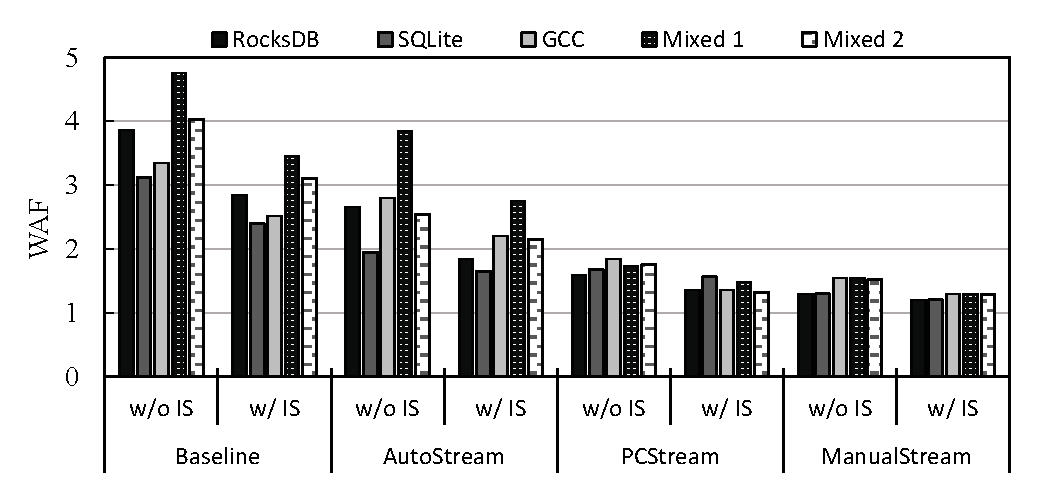
\includegraphics[width=1.\linewidth]{figure/internal}
	\caption{The effect of internal streams on WAF.}
	\vspace{-5pt}
	\label{fig:internal}
	\vspace{-10pt}
\end{figure}

\vspace{-10pt}
\subsection{Impact of the PC Attribute Table}
\vspace{-5pt}
As explained in Section 5, the PC attribute table is useful to maintain a
long-term history of applications' I/O behavior by exploiting the uniqueness of
a PC signature across different applications.   To evaluate the effect of the
PC attribute table on the efficiency of \textsf{\small PCStream}, we modified
the implementation of the PC attribute table so that the PC attribute table can
be selectively disabled on demands when a process terminates its execution.
For example, in the kernel compilation scenario with GCC, the PC attribute
table becomes empty after each kernel build is completed.  That is, the next
kernel build will start with no existing PC to stream mappings.


Fig.~\ref{fig:pctable} show how many requests are assigned to the default
$S_{0}$ stream over varying sizes of the PC attribute table.  Since $S_{0}$ is
used when no stream is assigned for an incoming write request, the higher the
ratio of requests assigned to $S_{0}$, the less effective the PC attribute
table.   As shown in Fig.~\ref{fig:pctable}, in RocksDB, Cassandra, and SQLite,
the PC attribute table did not affect much the ratio of writes on $S_{0}$.
This is because these programs run continuously for a long time while
performing the same dominant activities repeatedly.  Therefore, although the PC
attribute table is not maintained, they can quickly reconstruct it.  On the
other hand, the PC attribute table was effective for GCC, which frequently
creates and terminates multiple processes ({\it e.g.}, {\tt cc1}).  When no PC
attribute table was used, about 16\% of write requests were assigned to
$S_{0}$.  With the 4-KB PC attribute table, this ratio was reduced to 12\%.
With the 12-KB PC attribute table, only 9\% of write requests were assigned to
$S_{0}$.  This reduction in the $S_{0}$ allocation ratio reduced the WAF value
from 1.96 to 1.54.


